% Template for IGARSS-2018 paper; to be used with:
%          spconf.sty  - LaTeX style file, and
%          IEEEbib.bst - IEEE bibliography style file.
% --------------------------------------------------------------------------
\documentclass{article}
\usepackage{spconf,amsmath,epsfig}
\usepackage[hidelinks]{hyperref}
\usepackage{etoolbox}
\usepackage{textcomp}
% Example definitions.
% --------------------
\def\x{{\mathbf x}}
\def\L{{\cal L}}

\usepackage{scalerel}
\usepackage{tikz}
\usetikzlibrary{svg.path}

\definecolor{orcidlogocol}{HTML}{A6CE39}
\tikzset{
  orcidlogo/.pic={
    \fill[orcidlogocol] svg{M256,128c0,70.7-57.3,128-128,128C57.3,256,0,198.7,0,128C0,57.3,57.3,0,128,0C198.7,0,256,57.3,256,128z};
    \fill[white] svg{M86.3,186.2H70.9V79.1h15.4v48.4V186.2z}
                 svg{M108.9,79.1h41.6c39.6,0,57,28.3,57,53.6c0,27.5-21.5,53.6-56.8,53.6h-41.8V79.1z M124.3,172.4h24.5c34.9,0,42.9-26.5,42.9-39.7c0-21.5-13.7-39.7-43.7-39.7h-23.7V172.4z}
                 svg{M88.7,56.8c0,5.5-4.5,10.1-10.1,10.1c-5.6,0-10.1-4.6-10.1-10.1c0-5.6,4.5-10.1,10.1-10.1C84.2,46.7,88.7,51.3,88.7,56.8z};
  }
}

\newcommand\orcidicon[1]{\href{https://orcid.org/#1}{\mbox{\scalerel*{

\begin{tikzpicture}[yscale=-1,transform shape]
\pic{orcidlogo};
\end{tikzpicture}
}{|}}}}

% Title.
% ------
\title{FRESH SNOW DEPTH ESTIMATION USING SPACEBORNE X-BAND POLARIMETRIC SYNTHETIC APERTURE RADAR DATA}
%
% Single address.
% ---------------
\name{Sayantan Majumdar\textsuperscript{1,2} \orcidicon{0000-0002-3539-0147}\,, Praveen K. Thakur\textsuperscript{3}, Ling Chang\textsuperscript{1}, Shashi Kumar\textsuperscript{4}}
\address{\textsuperscript{1}Department of Earth Observation Science, Faculty of Geo-information Science and Earth Observation\\ (ITC), University of Twente, Enschede, The Netherlands\\
\textsuperscript{2}Geoinformatics Department, Indian Institute of Remote Sensing (IIRS), ISRO, Dehradun, India\\
\textsuperscript{3}Water Resources Department, Indian Institute of Remote Sensing (IIRS), ISRO, Dehradun, India \\
\textsuperscript{4}Photogrammetry and Remote Sensing Department, Indian Institute of Remote Sensing (IIRS), ISRO,\\ Dehradun, India\\
Email: \href{mailto: sayantan.majumdar@ieee.org}{sayantan.majumdar@ieee.org}, \href{mailto: praveen@iirs.gov.in}{praveen@iirs.gov.in}, \href{mailto: ling.chang@utwente.nl}{ling.chang@utwente.nl}, \href{mailto: shashi@iirs.gov.in}{shashi@iirs.gov.in} 
}
\tolerance=1
\emergencystretch=\maxdimen
\hyphenpenalty=10000
\hbadness=10000
\sloppy

\begin{document}
%\ninept
%
\maketitle
%
\begin{abstract}
The estimation of fresh snow depth (FSD) using X-band synthetic aperture radar (SAR) is feasible but challenging depending on the geological conditions and data availability. In this study, the FSD is computed for the Beas river watershed in the northwestern Himalayas near Manali, India. It incorporates the recent copolar phase difference (CPD) based FSD inversion model. Moreover, the TerraSAR-X and TANDEM-X bistatic data acquired in January 2016 are used as inputs to the model along with the snow density measurements at the Dhundi ground station. Additionally, apart from applying layover and forest masks, the potential uncertainty sources in the complex mountainous terrains are identified using the H-A-$\alpha$ decomposition and unsupervised Wishart classification techniques. Furthermore, due to the limited number of weather stations, the results are validated using a 3x3 neighbourhood window surrounding the Dhundi site. Also, the effect of different FSD ensemble window sizes are tested for performing sensitivity analysis.
\end{abstract}
%
\begin{keywords}
Fresh snow, synthetic aperture radar, copolar phase difference, polarimetry, snow anisotropy
\end{keywords}
%
\section{Introduction}
\label{sec:intro}
Snow depth or snow height is one of the most important physical properties of snow and finds extensive usage in hydrological models, particularly in snowmelt runoff and snow avalanche predictions \cite{Thakur2012}. Essentially, it represents the height of the snow surface from the ground underneath. Moreover, it is also used to measure the snow water equivalent (SWE) which quantifies the amount of water present in a snowpack \cite{Tedesco2015}. However, large-scale accurate snow depth estimation can be challenging depending on the availability of suitable data and the geological situations of the study area \cite{Leinss2014}.

In this regard, standard practice is to couple remote sensing techniques with adequately sampled spatiotemporal ground observations, thereby improving the quality of the resultant snow depth map \cite{Thakur2012}, \cite{Leinss2014}. Nowadays, Light Detection and Ranging (LiDAR) and Synthetic Aperture Radar (SAR) have been widely adopted for measuring snow depth with sufficiently high accuracies in the order of centimetres \cite{Tedesco2015}--\cite{Deems2013}. Although laser altimetry measurements offer high-quality results, the data acquisition is sensitive to weather conditions and is also expensive \cite{Deems2013}. Therefore, spaceborne SAR, which facilitates globally available high-resolution datasets along with weather independency and night-time operability, is extensively utilised in the cryospheric studies \cite{Thakur2012}, \cite{Leinss2014}, \cite{Moreira2013}.

Since snow is a porous birefringent medium which is a mixture of air, ice and water, the microwave interactions occurring at all these constituent phases need to be properly understood. For frequencies X-band and below, the major backscattering occurs at the snow-ground interface in case of dry snow, whereas surface scattering contributes the maximum when the snow is wet. However, humid snow exhibits a significant volume scattering which occurs within the snowpack \cite{Thakur2012}, \cite{Leinss2014}. In essence, the scattering mechanism is governed by the volumetric liquid water content of the snowpack which is responsible for controlling the microwave absorption in snow \cite{Leinss2014}.

In addition to this, the snow metamorphism induced anisotropy and snow density are critical factors which must be considered for estimating the fresh snow depth (FSD). X-Ray computer tomography scans have shown that in the initial stage, the freshly fallen snow exhibits a random structure which upon settling is transformed to horizontally aligned or oblate particles having snow densities in the range of 0.03-0.12 g/cm\textsuperscript{3}. Gradually, vertically shaped prolate particles (firn and depth hoar) are formed displaying snow density values in the order of 0.5 g/cm\textsuperscript{3}. After further recrystallisation, solid ice is produced whose density has been found to be 0.917 g/cm\textsuperscript{3} \cite{Leinss2014}, \cite{Riche2013}. Moreover, the effective permittivity ($\epsilon_{snow}$) of dry snow (fresh snow, firn, and depth hoar) is independent of the microwave frequency in the 10 MHz to 1 THz electromagnetic (EM) wave spectrum and only shows a strong dependence on the snow density \cite{Leinss2014}.

In principle, the three orthogonal axes ($a_x$, $a_y$, $a_z$) of a spheroid represented in the 3D ($x$, $y$, $z$) Cartesian coordinate system correspond to the three dipoles which essentially characterises the dielectric nature of an ice particle. This is highlighted in figure \ref{fig:prolate}, where a prolate ice particle is linked with the radar reference frame ($h$, $k$, $v$) following the radar backscattering alignment (BSA) convention. Here, $k$, $h$ and $v$ are the propagation vector, wave components of the horizontal and vertical polarisations respectively, $\theta$ being the satellite incidence angle obtained with respect to the surface normal \cite{Leinss2014}.

\AfterEndEnvironment{figure}{\vspace{-1ex}}
\begin{figure}[htb]
\centering
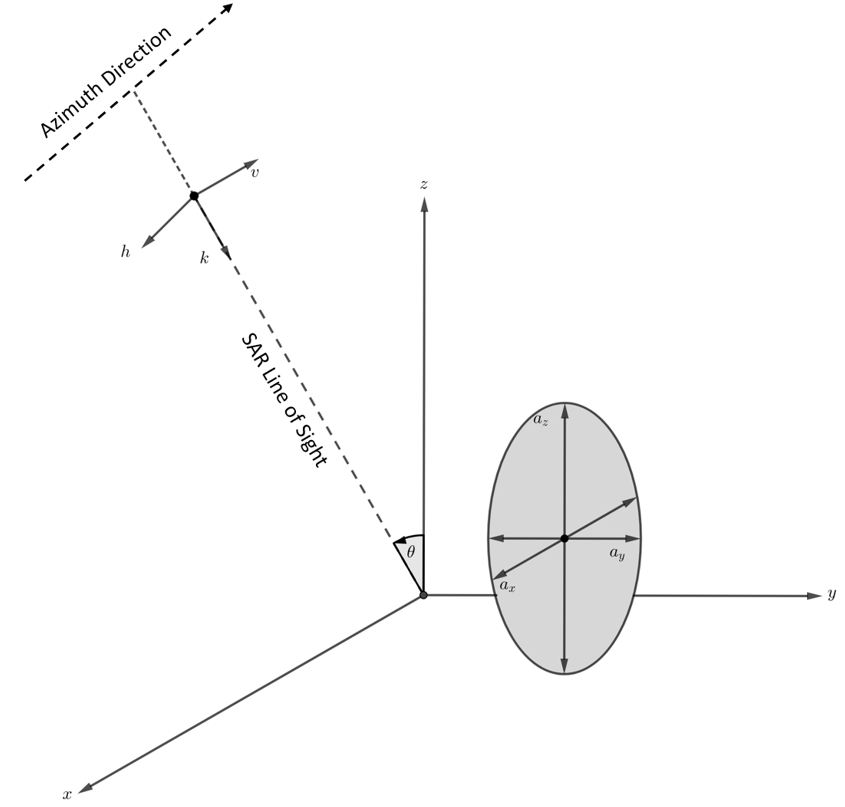
\includegraphics[scale=0.14]{Prolate_New.png}
\vspace{-2ex}
\caption{The orientation of a single prolate ice particle linked with the radar reference frame (adapted from \cite{Leinss2014}).}
\label{fig:prolate}
\end{figure}

Furthermore, the depolarisation factor is an important component to model the snow anisotropy which in turn, is used as a parameter in the FSD inversion algorithm based on the copolar phase difference (CPD) approach \cite{Leinss2014}. In this work, the CPD method is applied to compute the FSD in the complex alpine terrains of the Beas watershed, northwestern Himalayas. Additionally, due to the extreme geological conditions there exist significant uncertainty sources which are discussed explicitly in the later sections.

\section{Study area and Data}
\label{sec:study}
\subsection{Study Area}
\label{ssec:area}
The Beas river watershed near Manali, India is characterised by steep slopes and dense forests. The elevation varies from about 2500 m to more than 5000 m (figure \ref{fig:overview}). In this work, the Beas basin, starting from a few kilometres uphill from Dhundi up to Kothi (figure \ref{fig:overview}) has been chosen for FSD estimation. The areas surrounding Dhundi and Kothi receive significant seasonal snowfall usually from the onset of December to late March. However, the cold, dry season starts from as early as October. The coldest period is in January with temperatures reaching a mean daily minimum of -15\textsuperscript{0}C whereas, in June, mean and maximum temperatures of 20\textsuperscript{0}C and 30\textsuperscript{0}C respectively are commonly observed. Additionally, heavy rainfall occurs in the monsoon season (late June-September) with August being the wettest month \cite{Thakur2012}. In total, an area of approximately 130 km\textsuperscript{2} is depicted in Figure \ref{fig:overview} showing ALOS PALSAR digital elevation model (DEM). Here, the original 12.5 m DEM has been resampled to 3 m to match the high-resolution SAR data used in this research. 

\AfterEndEnvironment{figure}{\vspace{-3.5ex}}
\begin{figure}[htb]
\centering
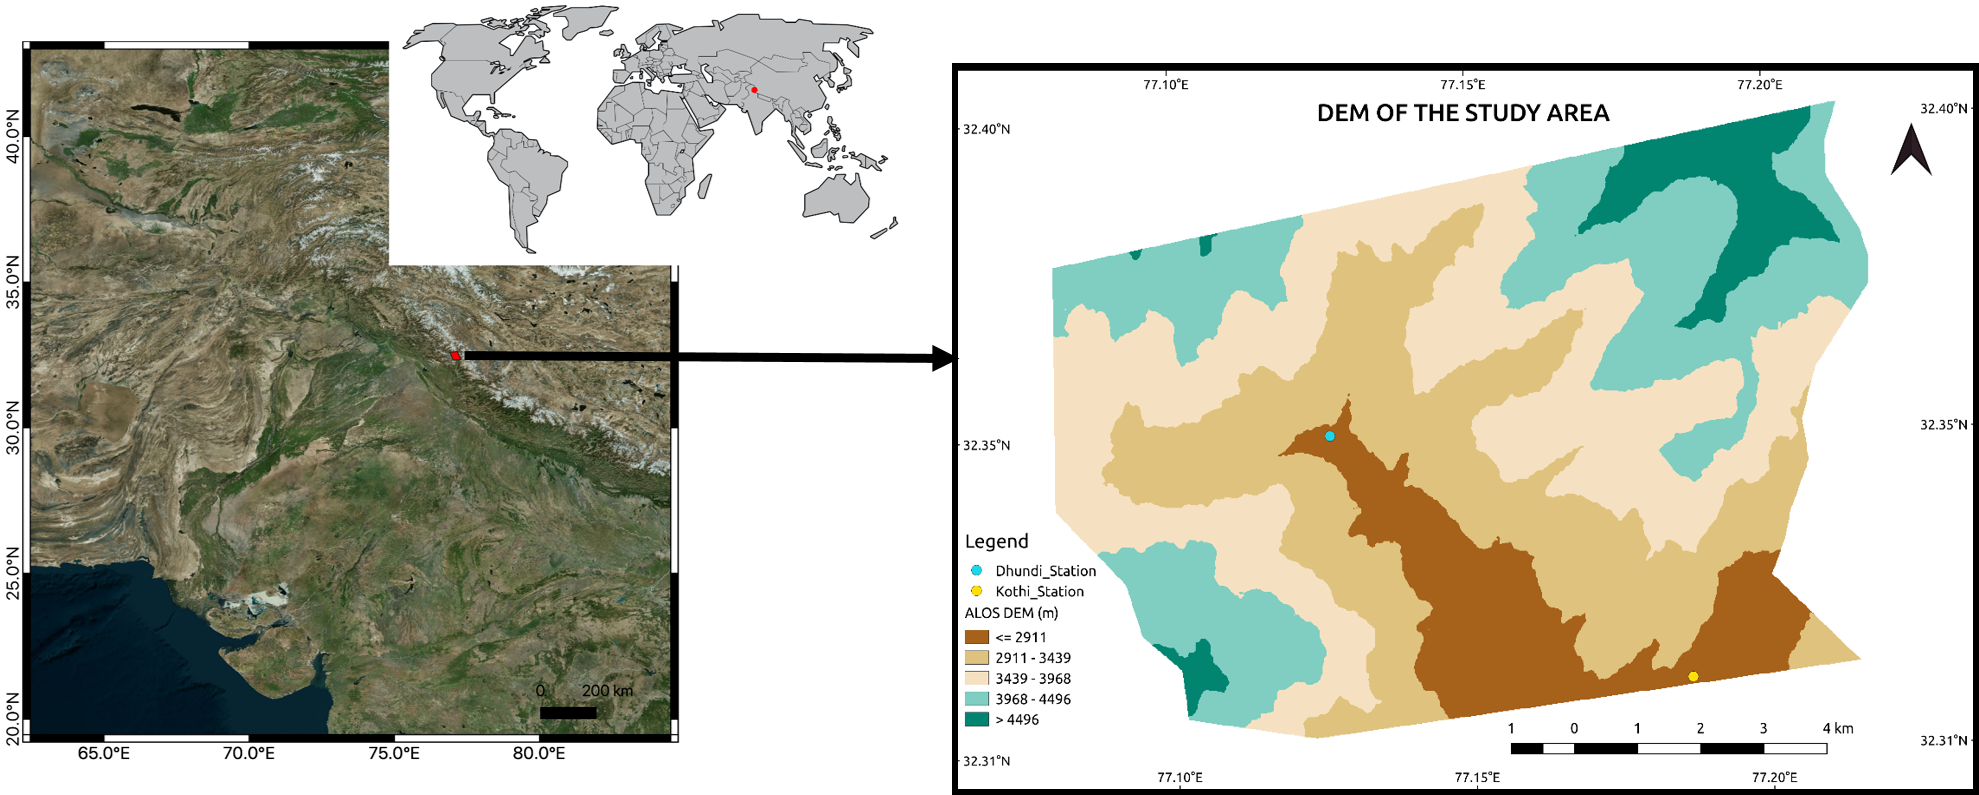
\includegraphics[scale=0.14]{Overview.png}
\vspace{-2ex}
\caption{The overview map of the study area showing the ALOS PALSAR DEM, Dhundi and Kothi ground stations.}
\label{fig:overview}
\end{figure}

\subsection{Available Datasets}
\label{ssec:data}
Regarding the SAR data, fully polarimetric (Quad-pol) and Coregistered Single look Slant range Complex (CoSSC) X-band bistatic acquisitions in stripmap (SM) mode from TerraSAR-X and TANDEM-X satellites have been used. Overall six Quad-pol data pairs were available, out of which the descending orbital pass acquisition at 00:53 hrs, Jan 8, 2016, has been selected considering the occurrence of fresh snowfall before, during and after the satellite flyby.

Additionally, intensive fieldwork had been conducted from Oct 14-21, 2018 in the Dhundi and Kothi areas where several differential GPS (DGPS) measurements were acquired with adequate positional accuracies ($\approx$7 cm). Moreover, the in-situ snow physical parameters’ data (total and fresh snow depths, snow density) along with the relevant weather data were transferred to a PostgreSQL database from the manual recordings. Accordingly, the fresh snow depths on the Jan 7, 2016 evening and Jan 8, 2016 morning were 5 cm and 22 cm respectively signifying a heavy snowfall event.

Apart from this, a Landsat 8 OLI acquisition over the study area on May 12, 2016 (summer season) had been downloaded to prepare the forest mask.    

\section{Methodology}
\label{sec:method}
The steps involved in this research workflow are depicted in figure \ref{fig:work}. All the processing tasks have been carried out using open-source tools and libraries which include the Sentinel Application Platform (SNAP), QGIS and Python.

At first, the CoSSC product has been split into separate TerraSAR-X, and TANDEM-X images and then radiometric calibration has been applied. After subsetting these images, the CPDs are computed individually using \eqref{1} where $\Im$ and $\Re$ denote the imaginary and real parts of the complex scattering matrices $S_{VV}$ and $S_{HH}$ respectively ($\phi_{VV}$ and $\phi_{HH}$ representing the corresponding phases), $\langle\rangle$ denoting the ensemble averaging operation. These are subsequently averaged to a single CPD image. Thereafter, terrain correction is performed using the ALOS PALSAR DEM where the local incidence angle (LIA) is also stored as an image band alongside CPD.

The geocoded CPD image (3 m spatial resolution) is then used as an input to the FSD estimation module written in Python. Initially, the CPD values are averaged based on an ensemble window of 5x5 pixels (225 m\textsuperscript{2} ground area). The FSD ($\Delta Z_f$) inversion model is given by \eqref{2} where the CPD ($\phi_{CPD}\in[-\pi,\pi]$), radar wavelength ($\lambda_0$), LIA ($\theta_l$), and the two snow refractive indices, $n_V$ and $n_H$ (corresponding to the two polarisations VV and HH respectively) are the involved parameters. In this regard, it has been found that for fresh snow,  $\phi_{CPD}>0$ and $n_H>n_V$, i.e., $\Delta{\zeta}<1$ \cite{Leinss2014}.
\AfterEndEnvironment{figure}{\vspace{2.5ex}}
\begin{figure}[htb]
\centering
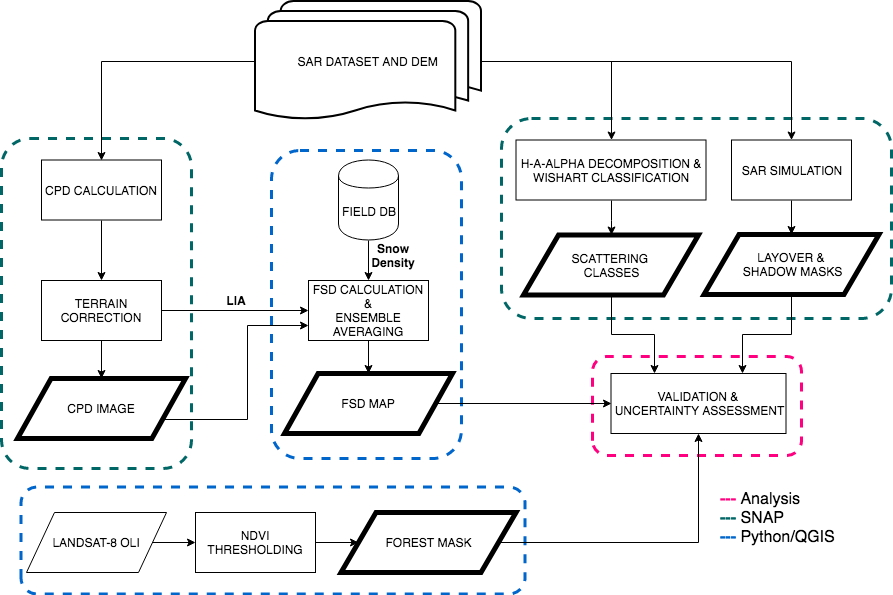
\includegraphics[scale=0.14]{Method_FSD.png}
\vspace{-2ex}
\caption{The research workflow highlighting the major tasks.}
\label{fig:work}
\end{figure}

Essentially, \eqref{2} is based on the underlying Maxwell-Garnett EM mixture model and the depolarisation factor equations, a detailed treatment of which is provided by \cite{Sihvola1999}. The estimated FSD values are further averaged using different square and rectangular ensemble windows after which the final map is prepared in QGIS.

\BeforeBeginEnvironment{equation}{\vspace{-2ex}}
\AfterEndEnvironment{equation}{\vspace{0.5ex}}
\begin{equation}\tag{1}
    \centering
    \small{\phi_{CPD} =\left\langle\underbrace{\tan^{-1}\left(\frac{\Im\left(S_{VV}\right)}{\Re\left(S_{VV}\right)}\right)}_{\phi_{VV}} - \underbrace{\tan^{-1}\left(\frac{\Im\left(S_{HH}\right)}{\Re\left(S_{HH}\right)}\right)}_{\phi_{HH}}\right\rangle}
    \label{1}
\end{equation}
\begin{equation}\tag{2}
    \centering
    \small{\Delta{Z_f} = (-1)\frac{\lambda_0\phi_{CPD}}{4\pi\Delta{\zeta}}}
    \label{2}
\end{equation}
\BeforeBeginEnvironment{equation*}{\vspace{-1ex}}
\begin{equation*}
    \centering
    \text{where } \small{\Delta{\zeta} = \sqrt{n^2_V - \sin^{2}\theta_l} - \sqrt{n^2_H - \sin^{2}\theta_l}}
\end{equation*}


In addition to this, the layover, shadow (SAR simulation) and forest masks (NDVI thresholding) are generated (3 m spatial resolution) to assess the potential uncertainty sources qualitatively. Moreover, the H-A-$\alpha$ decomposition and unsupervised Wishart classification techniques have been used to compare the scattering mechanisms in the study sites during snow-covered (Jan 8, 2016) and snow-free (Jun 8, 2017) seasons \cite{Singh2014}.     

\section{Results and Discussion}
\label{sec:results}
\subsection{Scattering Patterns}
\label{ssec:scat}
Although the Jan 8, 2016 data was quad-pol, the data acquired on Jun 8, 2017, had only HH and VV channels (dual-pol). As a result, the roll-invariant dual-pol entropy-anisotropy-$\alpha$ (H-A-$\alpha$) decomposition (5x5 window size) and unsupervised Wishart classification (10 iterations) have been performed for the snow-covered and snow-free periods \cite{Singh2014}. The classification results are shown in figures \ref{fig:wishart} (a) and (b) respectively wherein the increased volume scattering (from x\% to y\%) for January is clearly observable. Accordingly, there is a considerable reduction in the Brag surface scattering by z\% and also the double bounce scattering (occurring due to boulders and human establishments) is decreased from a\% to b\%. In this context, the ground observations show that there had been 20 mm rainfall on the evening of Jun 7, 2017, and since the satellite pass was at 00:53 hrs, the next day, the surface scattering effect is more prominent than double bounce scattering near the Dhundi site (figure \ref{fig:wishart} (b)). However, strong double bounce scattering is observable for the same region in the winter-time image.  

Moreover, the change in the scattering properties can also be verified with the corresponding H-$\alpha$ plane plots as shown in figures \ref{fig:wishart} (c) and (e) where the number of high entropy random anisotropic particles (snow indicator) increases while that of the medium entropy anisotropic particles (vegetation) decreases in the case of Jan 8, 2016.  
Furthermore, the non-feasible class represents the unclassified pixels occurring primarily due to the missing cross-pol SAR channels HV and VH. It can be seen that, for the summertime acquisition, the number of such unclassified pixels is significantly lower than that of the snow-covered period. The plausible reason for this could be attributed to the complex scattering mechanisms exhibited by the partially snow-covered vegetation features or boulders. In order to test this, the quad-pol H-A-$\alpha$ decomposition was applied on the winter-time image and there were no unclassified pixels (figure \ref{fig:wishart} (d)). Thus, the presence of snow causes a significant change of the scattering patterns in the study area resulting in significant uncertainty sources.

\AfterEndEnvironment{figure}{\vspace{-2ex}}
\begin{figure}[htb]
\centering
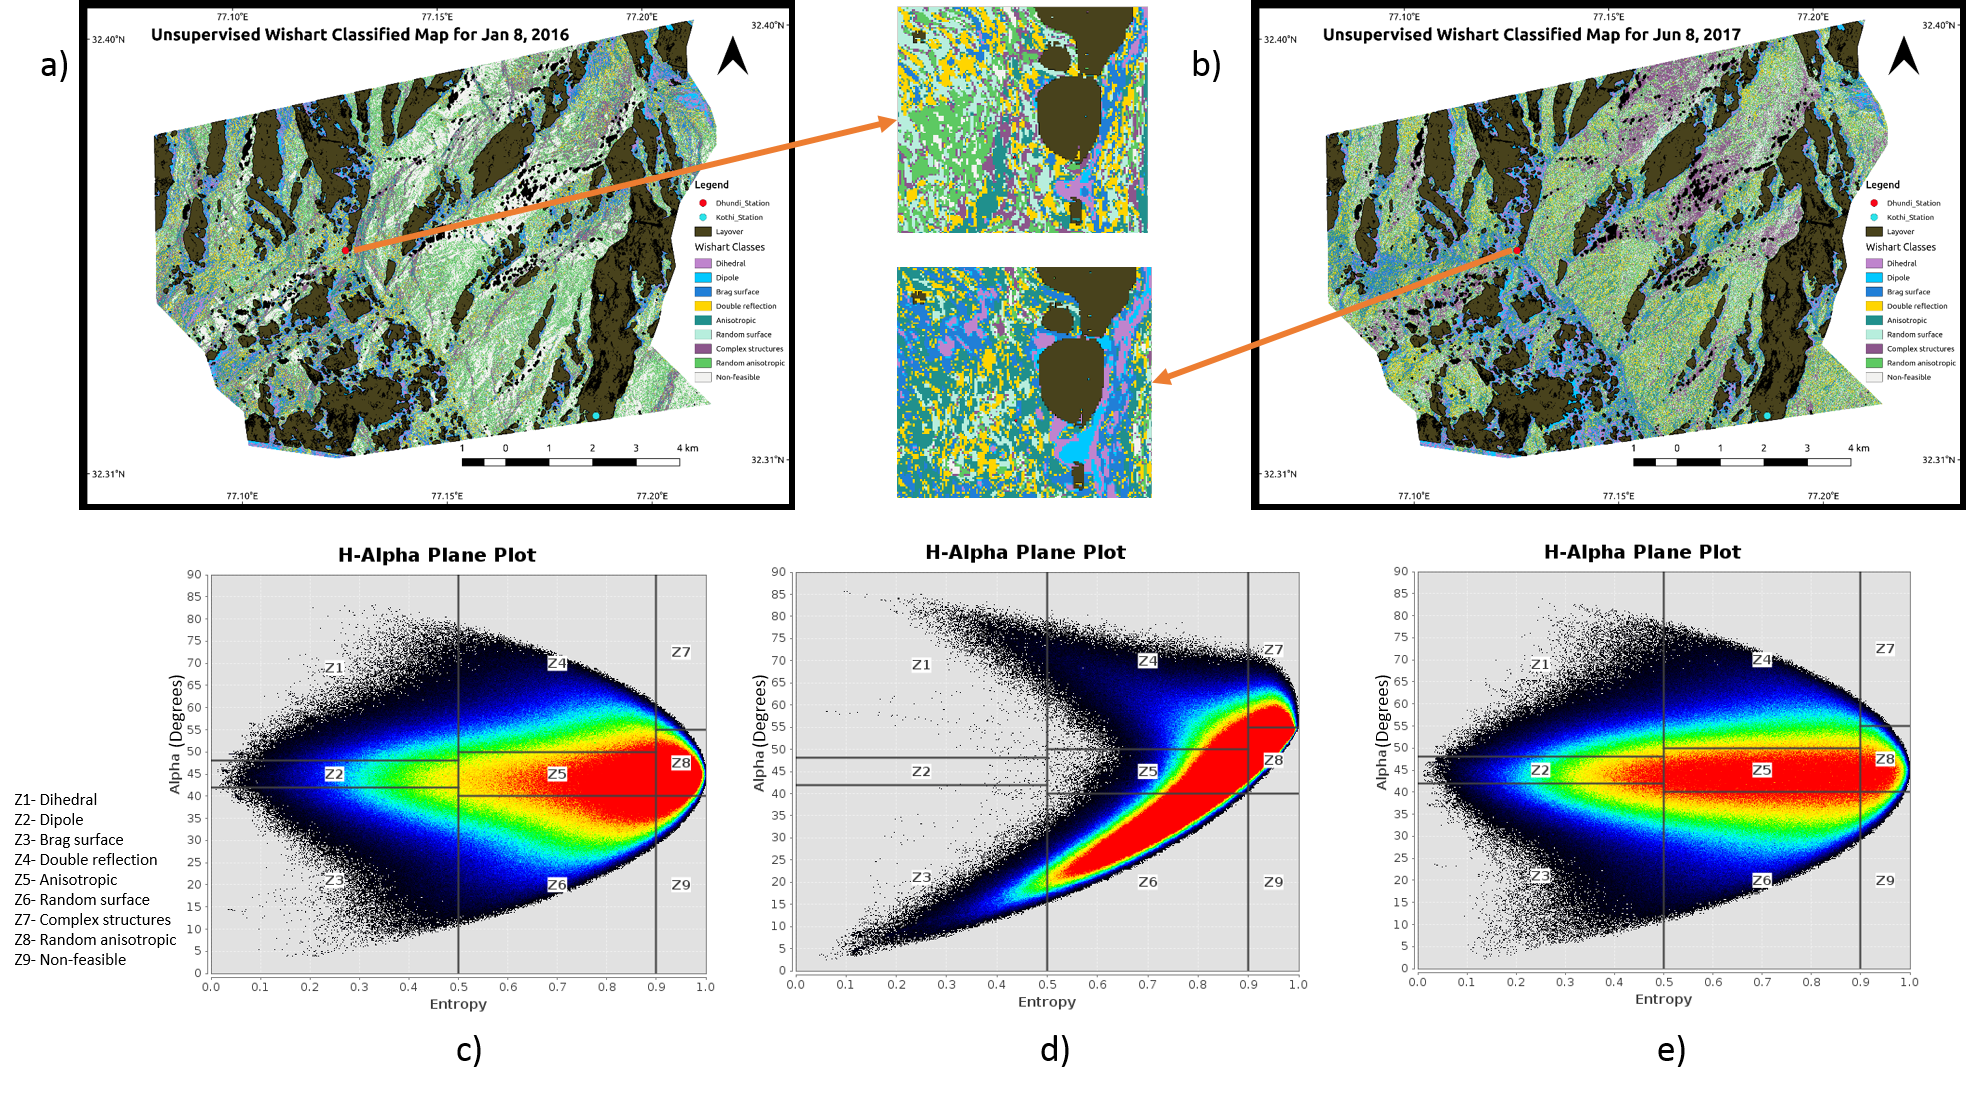
\includegraphics[scale=0.25]{All_Wishart.png}
\vspace{-2ex}
\caption{\textbf{(a)} Wishart classified maps and zoomed views for Jan 8, 2016 and \textbf{(b)} Jun 8, 2017 \textbf{(c)} Dual-pole H-$\alpha$ plot, Jan \textbf{(d)} Quad-pole H-$\alpha$ plot, Jan and \textbf{(e)} Dual-pole H-$\alpha$ plot, Jun.}
\label{fig:wishart}
\end{figure}

\subsection{Fresh Snow Depth Estimation}
\label{ssec:fsde}

The FSD has been estimated using the CPD based model described by \eqref{1} and \eqref{2} where the snow density for the entire study area has been set to 0.06 g/cm\textsuperscript{3} by considering the average of the Dhundi ground snow density measurements on Jan 7 and Jan 8, 2016. Moreover, the axial ratio ($e=a_x/a_z$) is assumed to be  0.2  following [3]\textquotesingle s work where $e \in (0,1)$ for prolate particles.

Here, the effect of different square and rectangular ensemble windows having step sizes of 10 and 1.19 respectively are tested. The subsequent graphical analyses over a 3x3 neighbourhood window surrounding the Dhundi site are shown in figures \ref{fig:fsd_map}{ (a) and (b)}. It can be seen that smaller window sizes result in either low mean FSD values ($\mu_f$) or high standard deviations ($\sigma_f$) which are essentially caused by the criteria enforced on $\phi_{CPD}$ and $\Delta{\zeta}$ in the FSD inversion model. In the Python implementation, $\Delta{Z_f} = 0 \, \forall \, \phi_{CPD} \le 0 \text{ or } \Delta{\zeta} \ge 1$ and therefore, larger window sizes are required to achieve suitable results which are in concordance with the ground truth data. Evidently, in case of the 5x5 ensemble window, $\mu_f \approx$ 0.006 cm (significantly low) and $\sigma_f \approx$ 0.02 cm, whereas for the 5x7 window, $\mu_f \approx$ 1.4 cm and $\sigma_f \approx$ 1.89 cm (quite high). As a result, determining an adequate window shape and size is an important task in this regard.

The final FSD map produced from the 65x65 ensemble window ($\approx$0.38 km\textsuperscript{2} ground area) is depicted in figure \ref{fig:fsd_map} (c) wherein $\mu_f \approx$ 8.95 cm and $\sigma_f \approx$ 0.09 cm. The corresponding histogram for the whole study area is also shown in figure 5 (d). Since the in-situ FSD measurement during the satellite pass lies between 5 cm and 22 cm, the estimated $\mu_f$ is justifiable. Although, larger window sizes were also providing sufficiently accurate results, in practical terms, averaging areas more than 0.4 km\textsuperscript{2} over such complex topographically varying terrains is unrealistic.
\AfterEndEnvironment{figure}{\vspace{0.4ex}}
\begin{figure}[htb]
\centering
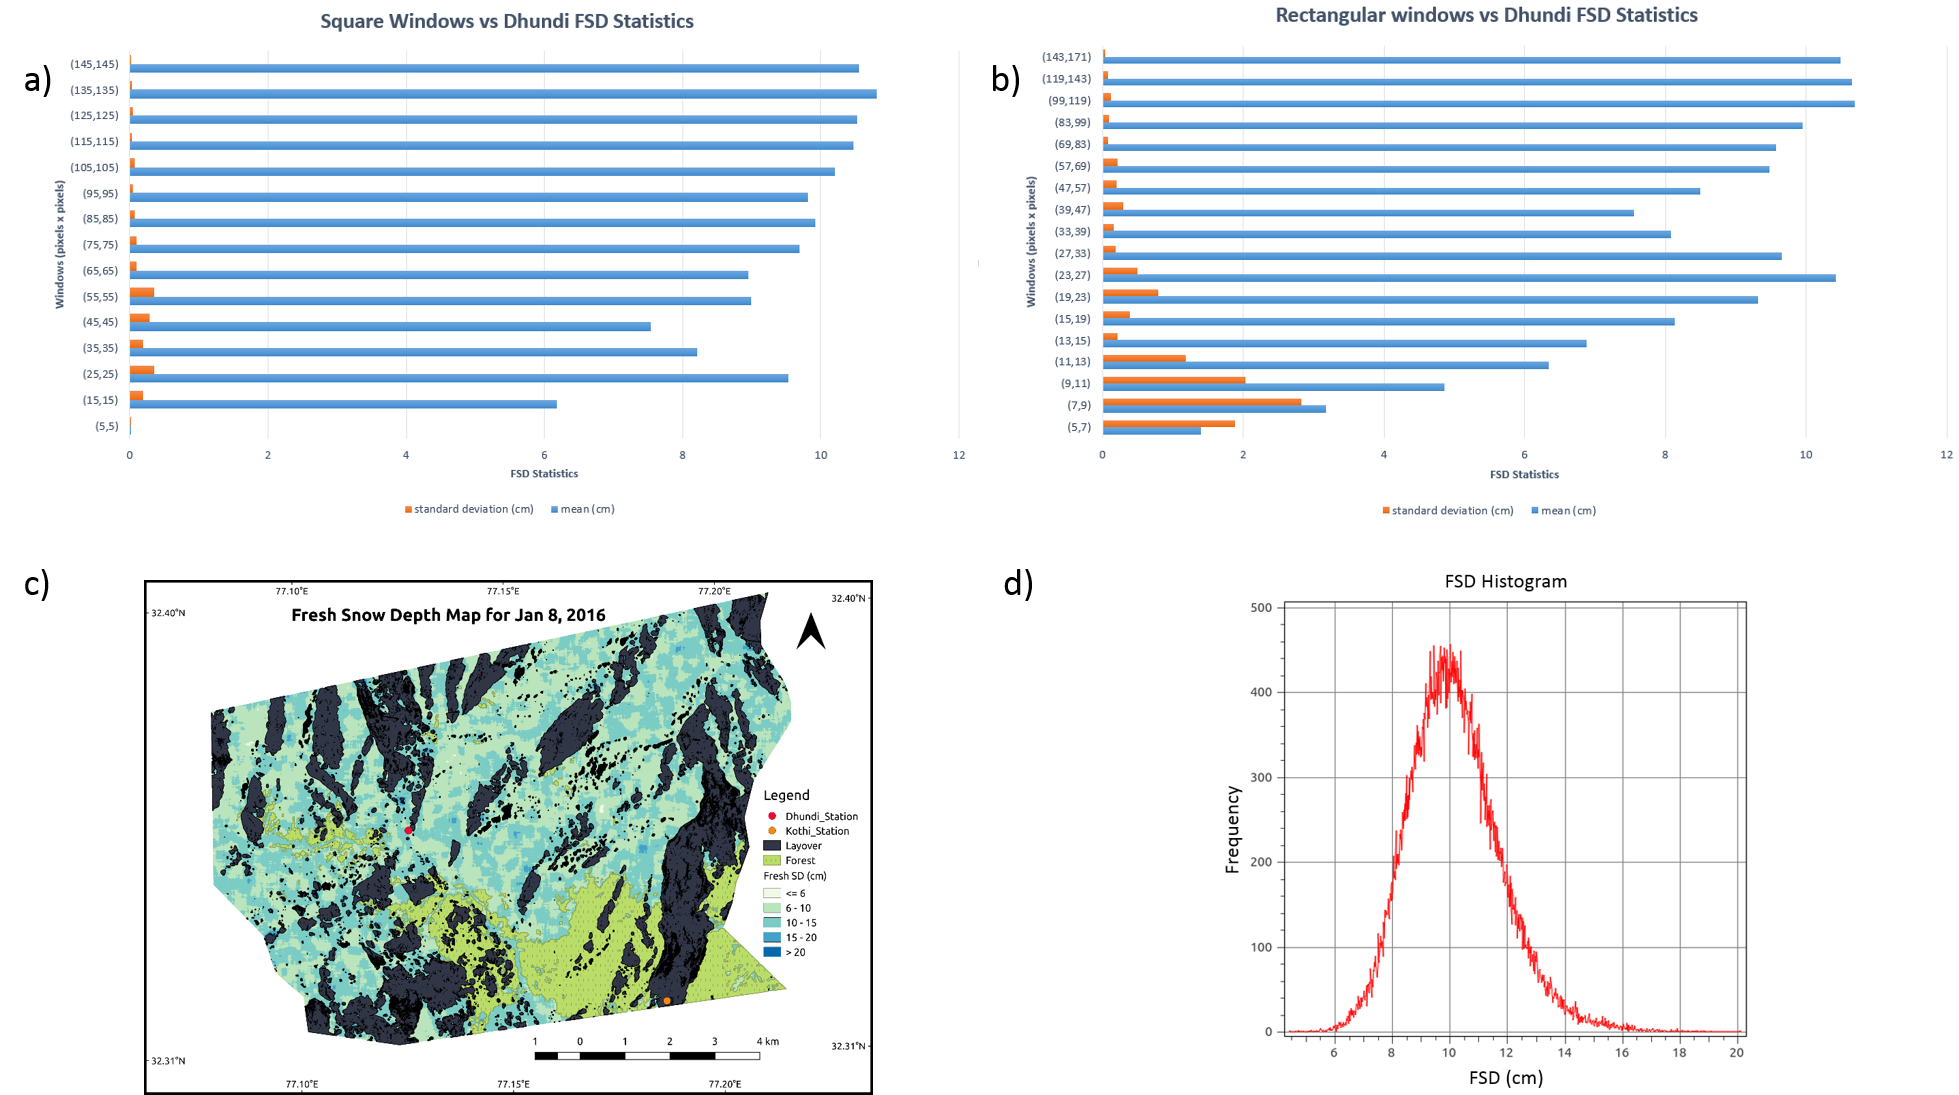
\includegraphics[scale=0.25]{All.png}
\vspace{-2ex}
\caption{\textbf{(a)} Square window and \textbf{(b)} Rectangular window statistics \textbf{(c)} FSD Map and \textbf{(d)} FSD histogram.}
\label{fig:fsd_map}
\end{figure}

\section{Conclusion}
\label{sec:concl}
In this work, an effort has been made for the first time to estimate the fresh snow depth in the presence of complex topographical features having significant uncertainty sources. In essence, the radar backscattering properties of these scatterers have been quantified with the dual-pol H-A-$\alpha$ decomposition and unsupervised Wishart classification techniques. Moreover, a comparative analysis has been performed for the snow-free and snow-covered seasons which showed that snow plays a critical role in significantly altering the scattering mechanisms. 

Also, the shape and size of the ensemble windows are the key factors for achieving sufficiently accurate and precise estimates. However, due to the limited ground stations, the field observations from only Dhundi had been used. This necessitated the consideration of a single snow density value across the entire study area, which is impractical.

Therefore, it is recommended to incorporate snow density variations along with the quantitative assessment of the ice particle axial ratio for potential future improvements. Furthermore, different windows have been tested for the FSD values only and hence, the ensemble window size effect on the CPD needs to be further investigated. Additionally, optical datasets such as Sentinel-2 images could be used in conjunction with the SAR imagery to obtain better snow cover maps which delineate dry and wet snow types.  Apart from this, other fully polarimetric SAR acquisitions offering high penetration capability such as the ALOS2-PALSAR2 L-band data could be used for subsequent studies in this regard. 


% References should be produced using the bibtex program from suitable
% BiBTeX files (here: strings, refs, manuals). The IEEEbib.bst bibliography
% style file from IEEE produces unsorted bibliography list.
% -------------------------------------------------------------------------
\bibliographystyle{IEEEbib}
\bibliography{IEEEabrv,refs}

\end{document}
